\section{Kunh Poker}

Este juego fue descrito en la sección \ref{section:kuhn-poker}. A diferencia de los juegos anteriores, es un juego secuencial, por lo que su representación natural es en forma extensiva. Sin embargo, como se mostró en la sección \ref{section:normal-extensiva}, todo juego en forma extensiva puede ser representado en forma normal, por lo que se pueden aplicar los algoritmos a al forma normal correspondiente.

En este juego, el jugador $2$ tiene una ganancia esperada de $\frac{1}{18}$ por mano, como se prueba en \cite{bib:kuhn-poker}. Además, el primer jugador tiene infinitas estrategias óptimas, las cuales pueden ser representadas por la elección de un parámetro $\alpha \in [ 0, \frac{1}{3} ]$. Una vez elegido este parámetro, en la primera jugada del primer jugador, este apuesta con probabilidad $\alpha$ cuando su carta tenga el número $1$, apuesta con una probabilidad $3 \alpha$ cuando tiene el número $3$ y siempre pasa cuando tiene el número $2$. Si el primer jugador tiene un segundo turno, debe pasar siempre que tenga el número $1$, apostar cuando tiene el número $3$, y en el caso que tenga el número $2$ debe apostar con probabilidad $\alpha + \frac{1}{3}$.

El segundo jugador tiene una única estrategia mixta óptima: apostar siempre que tenga el número $3$. Cuando tenga el número $1$, pasar siempre que el primer jugador haya apostado y apostar con probabilidad $\frac{1}{3}$ en caso contrario. Cuando tenga el número $2$, debe pasar cuando el oponente haya pasado previamente y apostar con probabilidad $\frac{2}{3}$ en caso contrario. La figura \ref{fig:kunh-poker-estrategias} muestra el árbol con las distribuciones de probabilidad de las estrategias previamente descritas en cada uno de los nodos alcanzables en el juego.

\begin{figure}[ht]
\begin{center}
\caption{Equilibrio de Nash del juego de Kunh poker}
\label{fig:kunh-poker-estrategias}
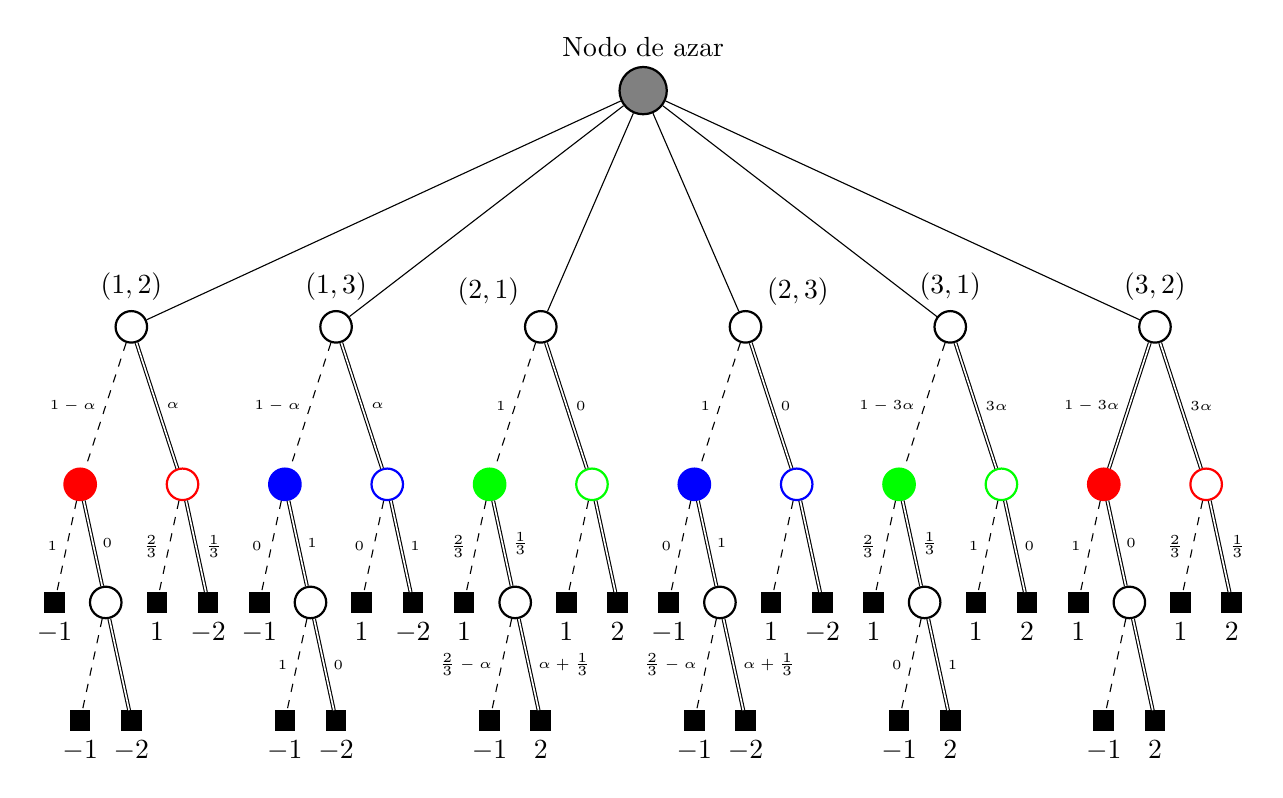
\begin{tikzpicture}[
chance/.style={circle, draw=black, fill=gray, thick, minimum size = 6mm},
player1/.style={circle, draw=black, solid, thick, minimum size = 4mm},
player2/.style={circle, thick, minimum size=4mm},
terminal/.style={rectangle, draw=black, solid, fill=black, thick, minimum size=2mm},
level 1/.style={sibling distance=26mm, level distance=30mm},
level 2/.style={sibling distance=13mm, level distance=20mm},
level 3/.style={sibling distance=6.5mm, level distance=15mm},
]
\node[chance] [label=above:{Nodo de azar}] {} {
	child {node [player1] (P1) [label=above:{$(1, 2)$}]{}
		child { node [player2] [draw=red, fill=red] {} 
				child { node [terminal] [label=below:{$-1$}] {}
						edge from parent [dashed] node [left, draw=none] {\tiny{$1$}} {} }
				child { node [player1] (A) {} 
						child { node [terminal] [label=below:{$-1$}] {}
								edge from parent [dashed] {} }
						child { node [terminal] [label=below:{$-2$}] {} 
								edge from parent [solid, double] {} }
						edge from parent [solid, double] node [right, draw=none] {\tiny{$0$}}  {}
				}
				edge from parent [dashed] node [left, draw=none] {\tiny{$1-\alpha$}}  {}
		}
		child { node [player2] [draw=red] {} 
				child { node [terminal] [label=below:{$1$}] {}
						edge from parent [dashed] node [left, draw=none] {\tiny{$\frac{2}{3}$}} {} }
				child { node [terminal] [label=below:{$-2$}] {}
						edge from parent [solid, double] node [right, draw=none] {\tiny{$\frac{1}{3}$}} {} }
				edge from parent [solid, double] node [right, draw=none] {\tiny{$\alpha$}}{}
		}
	}
	child {node [player1] (P2) [label=above:{$(1, 3)$}]{}
		child { node [player2] [draw=blue, fill=blue] {} 
				child { node [terminal] [label=below:{$-1$}] {}
						edge from parent [dashed] node [left, draw=none] {\tiny{$0$}} {} }
				child { node [player1] (B) {} 
						child { node [terminal] [label=below:{$-1$}] {}
								edge from parent [dashed] node [left, draw=none] {\tiny{$1$}} {} }
						child { node [terminal] [label=below:{$-2$}] {}
								edge from parent [solid, double] node [right, draw=none] {\tiny{$0$}} {} }
						edge from parent [solid, double] node [right, draw=none] {\tiny{$1$}} {}
				}
				edge from parent [dashed] node [left, draw=none] {\tiny{$1-\alpha$}} {}
		}
		child { node [player2] [draw=blue] {} 
				child { node [terminal] [label=below:{$1$}] {}
						edge from parent [dashed] node [left, draw=none] {\tiny{$0$}} {} }
				child { node [terminal] [label=below:{$-2$}] {}
						edge from parent [solid, double] node [right, draw=none] {\tiny{$1$}} {} }
				edge from parent [solid, double] node [right, draw=none] {\tiny{$\alpha$}} {}
		}
	}
	child {node [player1] (P3) [label=135:{$(2, 1)$}]{}
		child { node [player2] [draw=green, fill=green] {} 
				child { node [terminal] [label=below:{$1$}] {}
						edge from parent [dashed] node [left, draw=none] {\tiny{$\frac{2}{3}$}} {} }
				child { node [player1] (C) {} 
						child { node [terminal] [label=below:{$-1$}] {}
								edge from parent [dashed] node [left, draw=none] {\tiny{$\frac{2}{3}-\alpha$}} {} }
						child { node [terminal] [label=below:{$2$}] {} 
                        		edge from parent [solid, double] node [right, draw=none] {\tiny{$\alpha+\frac{1}{3}$}} {} }
						edge from parent [solid, double] node [right, draw=none] {\tiny{$\frac{1}{3}$}} {}
				}
				edge from parent [dashed] node [left, draw=none] {\tiny{$1$}} {}
		}
		child { node [player2] [draw=green] {} 
				child { node [terminal] [label=below:{$1$}] {}
						edge from parent [dashed] {} }
				child { node [terminal] [label=below:{$2$}] {}
						edge from parent [solid, double] {} }
				edge from parent [solid, double] node [right, draw=none] {\tiny{$0$}} {}
		}
	}
	child {node [player1] (P4) [label=45:{$(2, 3)$}]{}
		child { node [player2] [draw=blue, fill=blue]{} 
				child { node [terminal] [label=below:{$-1$}] {}
						edge from parent [dashed] node [left, draw=none] {\tiny{$0$}} {} }
				child { node [player1] (D) {} 
						child { node [terminal] [label=below:{$-1$}] {}
								edge from parent [dashed] node [left, draw=none] {\tiny{$\frac{2}{3}-\alpha$}} {} {} }
						child { node [terminal] [label=below:{$-2$}] {}
								edge from parent [solid, double] {} node [right, draw=none] {\tiny{$\alpha+\frac{1}{3}$}} {} }
						edge from parent [solid, double] node [right, draw=none] {\tiny{$1$}} {}
				}
				edge from parent [dashed] node [left, draw=none] {\tiny{$1$}} {}
		}
		child { node [player2] [draw=blue] {} 
				child { node [terminal] [label=below:{$1$}] {}
						edge from parent [dashed] {} }
				child { node [terminal] [label=below:{$-2$}] {}
						edge from parent [solid, double] {} }
				edge from parent [solid, double] node [right, draw=none] {\tiny{$0$}} {}
		}
	}
	child {node [player1] (P5) [label=above:{$(3, 1)$}]{}
		child { node [player2] [draw=green, fill=green] {} 
				child { node [terminal] [label=below:{$1$}] {}
						edge from parent [dashed] node [left, draw=none] {\tiny{$\frac{2}{3}$}} {} }
				child { node [player1] (E) {} 
						child { node [terminal] [label=below:{$-1$}] {}
								edge from parent [dashed] node [left, draw=none] {\tiny{$0$}} {} }
						child { node [terminal] [label=below:{$2$}] {}
								edge from parent [solid, double] node [right,draw=none] {\tiny{$1$}} {} }
						edge from parent [solid, double] node [right, draw=none] {\tiny{$\frac{1}{3}$}} {}
				}
				edge from parent [dashed] node [left, draw=none] {\tiny{$1-3 \alpha$}} {}
		}
		child { node [player2] [draw=green] {} 
				child { node [terminal] [label=below:{$1$}] {}
						edge from parent [dashed] node [left, draw=none] {\tiny{$1$}} {} }
				child { node [terminal] [label=below:{$2$}] {}
						edge from parent [solid, double] node [right, draw=none] {\tiny{$0$}} {} }
				edge from parent [solid, double] node [right, draw=none] {\tiny{$3 \alpha$}} {}
		}
	}
	child {node [player1] (P6) [label=above:{$(3, 2)$}]{}
		child { node [player2]  [draw=red, fill=red] {} 
				child { node [terminal] [label=below:{$1$}] {}
						edge from parent [dashed] node [left, draw=none] {\tiny{$1$}} {} }
				child { node [player1] (F) {} 
						child { node [terminal] [label=below:{$-1$}] {}
								edge from parent [dashed] {}}
						child { node [terminal] [label=below:{$2$}] {}
								edge from parent [solid, double] {} }
						edge from parent [solid, double] node [right, draw=none] {\tiny{$0$}} {}
				}
				edge from parent [solid, double] node [left, draw=none] {\tiny{$1-3\alpha$}} {}
		}
		child { node [player2]  [draw=red] {} 
				child { node [terminal] [label=below:{$1$}] {}
						edge from parent [dashed] node [left, draw=none] {\tiny{$\frac{2}{3}$}} {} }
				child { node [terminal] [label=below:{$2$}] {}
						edge from parent [solid, double] node [right, draw=none] {\tiny{$\frac{1}{3}$}} {} }
				edge from parent [solid, double] node [right, draw=none] {\tiny{$3\alpha$}} {}
		}
	}
};
\end{tikzpicture}
\end{center}
\end{figure}


\subsection{Detalles de Implementación}
Para obtener la representación del árbol de forma legible para la clase \textit{Nodo}, se creó un programa que simulara todos los juegos posibles utilizando \textit{dfs},los conjuntos de información fueron representados por un \textit{string} en el que el primer caracter es un número del $1$ al $3$ seguido por una secuencia formada por $p$ o $b$, según la historia del juego. Los conjuntos de información son enumerados según el orden en el que aparecen y para determinar si un conjunto de información ya se enumeró previamente se utiliza una tabla de \textit{hash} (de la librería estándar del lenguaje).

\subsection{Resolver el Juego Kuhn Poker}

Para resolver este juego se utilizó el procedimiento de Regret Matching con \textit{regret} incondicional, el cual es el más eficiente de los $3$ procedimientos descritos. Sin embargo, para poder aplicar este algoritmo es necesario llevar el juego a su forma normal, como se describe en la sección \ref{subsec:FN-FE}. Se realizó una corrida para obtener una estrategia hasta obtener un \textit{regret} menor que $10^{-5}$. El tiempo total fue de $3707.72$ segundos, y el número total de iteraciones fue de $535296954$. La Figura \ref{fig:regret-kuhn-poker} muestra el \textit{regret} con respecto al número de iteraciones. Se observa la convergencia a cero para ambos parámetros cuando el número de iteraciones tiende a infinito.

\begin{figure}[ht]
\caption{Gráfica del \textit{regret} con respecto al número de iteraciones del juego Kuhn Poker}
\label{fig:regret-kuhn-poker}
\centering
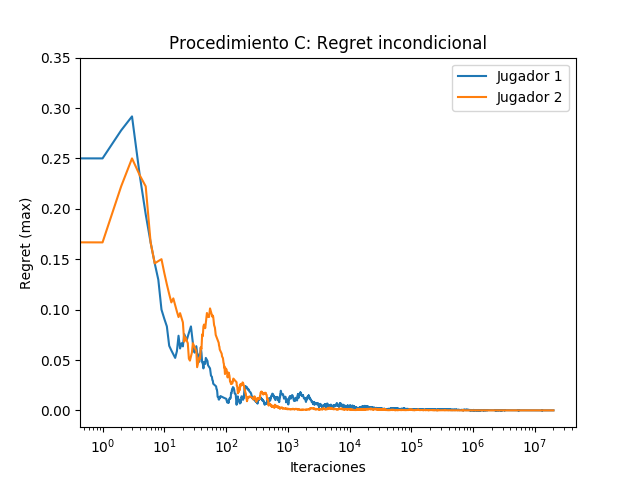
\includegraphics[width=0.5\textwidth]{graficas/kuhn/procedimiento-C.png}
\end{figure}

Para mostrar la estrategia obtenida, es necesario encontrar una estrategia de comportamiento equivalente a la estrategia mixta obtenida del algoritmo de \textit{Regret Matching}, como se describe en la sección \ref{subsec:EC-EM}. La Tabla \ref{tab:estrategia-kuhn-poker} muestra el equilibrio de Nash (parametrizado con la variable $\alpha$) y la estrategia obtenida del procedimiento. Se puede observar que la estrategia obtenida aproxima a un equilibrio de Nash con $\alpha \approx 0.249125$.

\begin{table}[ht]
    \centering
    \begin{tabular}{c|r r| r r}
        I & \multicolumn{2}{|c|}{Equilibrio de Nash} & \multicolumn{2}{|c}{Regret Matching} \\ \hline
         $1$ & $1-\alpha$ & $\alpha$ & $0.750875$ & $0.249125$ \\
         $2$ & $1$ & $0$ & $1$ & $0$ \\
         $3$ & $1$ & $0$ & $1$ & $0$ \\
         $4$ & $\frac{2}{3}$& $\frac{1}{3}$ & $0.666633$ & $0.333367$ \\
         $5$ & $0$ & $1$ & $0$ & $1$ \\
         $6$ & $1$ & $0$ & $1$ & $0$ \\
         $7$ & $0$ & $1$ & $0$ & $1$ \\
         $8$ & $\frac{2}{3}$ & $\frac{1}{3}$ & $0.666633$ & $0.333367$ \\
         $9$ & $\frac{2}{3} - \alpha$ & $\alpha + \frac{1}{3}$ & $0.417775$ & $0.582225$ \\
        $10$ & $1$ & $0$ & $1$ & $0$ \\
        $11$ & $1 - 3 \alpha$ & $3 \alpha$ & $0.253224$ & $0.746776$ \\
        $12$ & $0$ & $1$ & $0$ & $1$ \\ \hline
    \end{tabular}
    \caption{Equilibrio de Nash y estrategia obtenida para el juego de Kuhn Poker}
    \label{tab:estrategia-kuhn-poker}
\end{table}

Con la estrategia calculada se obtiene que peor caso para el primer jugador es igual a $v_1 = -0.0556501$ y el peor caso para el segundo jugador es $v_2 = 0.0555501$. Estos valores están bastantes cercas a la ganancia esperada cuando se utiliza el equilibrio de Nash, que es $-1/18$ y $1/18$, respectivamente. Se puede notar que la diferencia entre la ganancia esperada utilizando un equilibrio de Nash y la obtenida con las ganancias utilizadas es no mayor a $10 ^ {-4}$.
